\documentclass[default]{beamer}
\setbeamertemplate{navigation symbols}{}

\usetheme{CambridgeUS}
\useoutertheme{infolines}
%\usecolortheme{crane}

\usepackage{cmap}							% Поддержка поиска русских слов в PDF (pdflatex)
\usepackage[T2A]{fontenc}       			%поддержка кириллицы
\usepackage[utf8]{inputenc}					% Выбор языка и кодировки
\usepackage[english, russian]{babel}
\usepackage{tikz}
\usetikzlibrary{calc,patterns,backgrounds}

\graphicspath{{../../images/}} 			% Пути к изображениям

\makeatletter
\setbeamertemplate{footline}
{
	\leavevmode%
	\hbox{%
		\begin{beamercolorbox}[wd=.333333\paperwidth,ht=2.25ex,dp=1ex,center]{author
				in head/foot}%
			\usebeamerfont{author in
				head/foot}\insertshortauthor~~\beamer@ifempty{\insertshortinstitute}{}{(\insertshortinstitute)}
		\end{beamercolorbox}%
		\begin{beamercolorbox}[wd=.333333\paperwidth,ht=2.25ex,dp=1ex,center]{title in
				head/foot}%
			\usebeamerfont{title in head/foot}\insertshorttitle
		\end{beamercolorbox}%
		\begin{beamercolorbox}[wd=.333333\paperwidth,ht=2.25ex,dp=1ex,right]{date in
				head/foot}%
			\usebeamerfont{date in head/foot}\insertshortdate{}\hspace*{2em}
			\insertframenumber{}\hspace*{2ex} 
		\end{beamercolorbox}
	}%
	\vskip0pt%
}

\let\Theorem\relax
\newtheorem{Theorem}{Теорема}
\newtheorem{Def}{Определение}

\newcommand{\blockp}[3]{
	\node[draw, rectangle, pattern = #3, minimum width = #1, minimum height = #2] 
}

\begin{document}
	
	\title[Представление знаний, группа БПЛА]{Представление знаний в задачах согласованного перемещения группы БПЛА}
	\author[Панов]{Александр Панов\\н.~с., к.ф.-м.н.}
	\institute[ФИЦ ИУ РАН]{Федеральный исследовательский центр <<Информатика и управление>> РАН}
	\date{09 октября 2015~г.} 
	
	\begin{frame}
		\titlepage
	\end{frame}
	
	\begin{frame}
		\frametitle{Архитектура управления STRL}
		
		\begin{figure}
			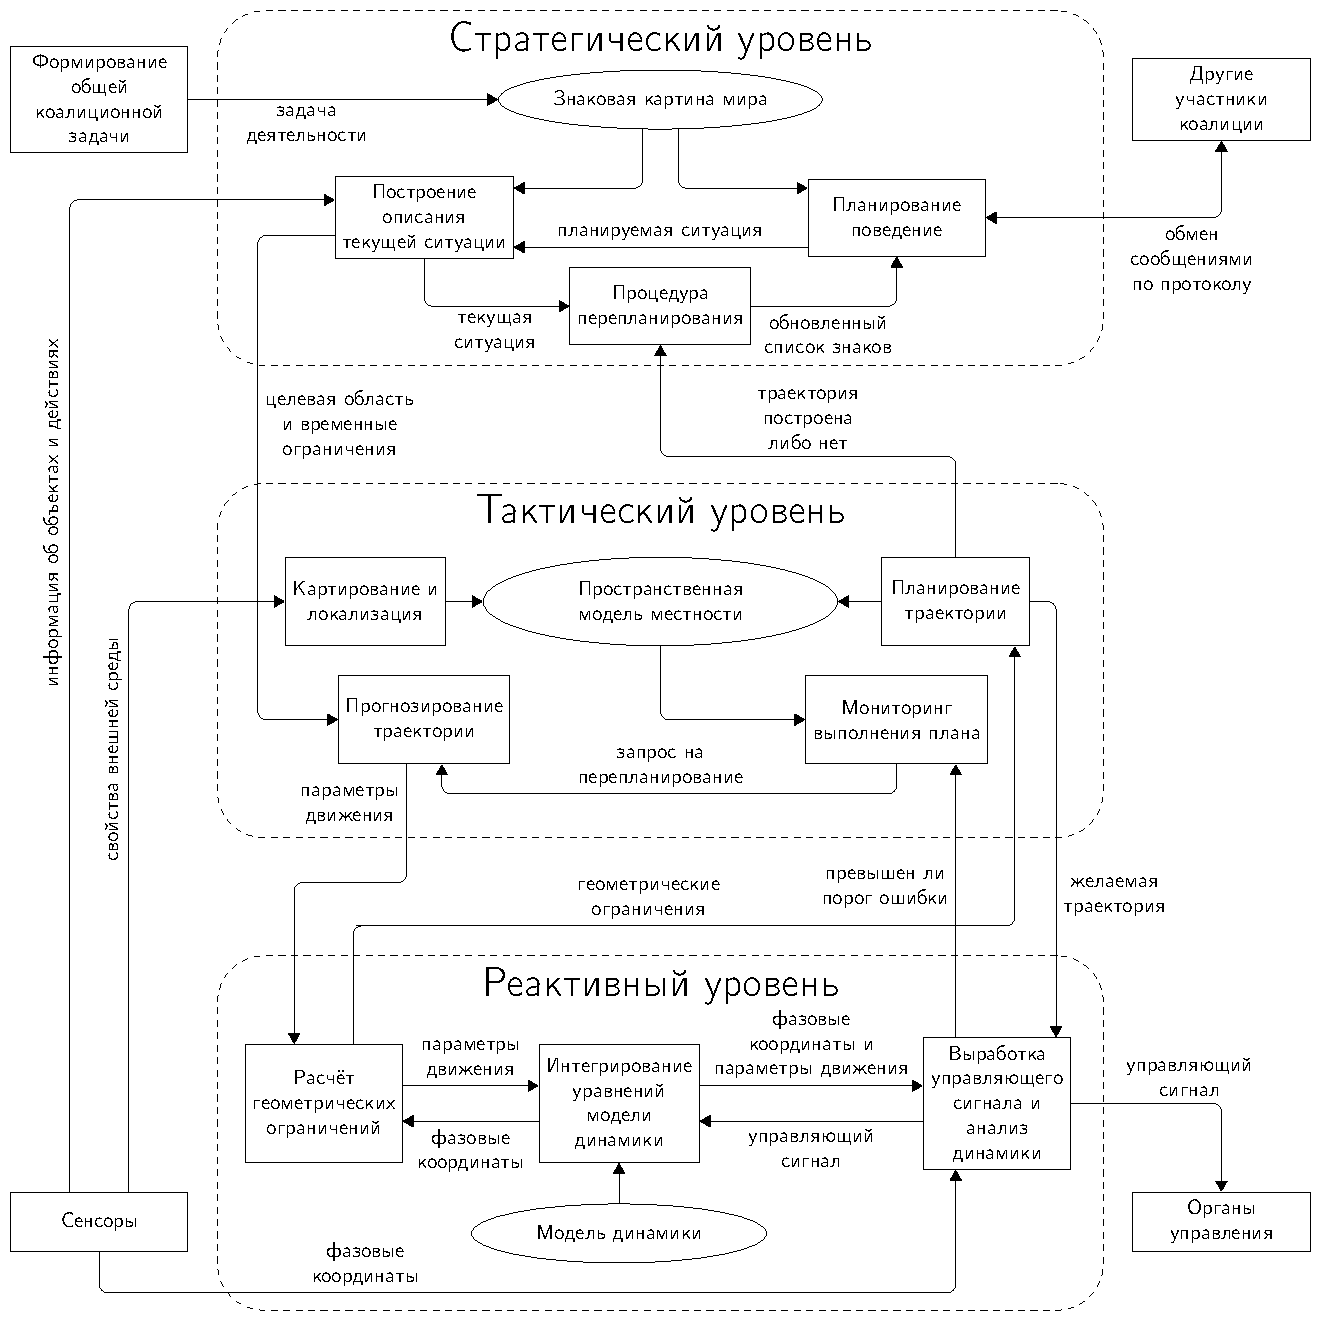
\includegraphics[width=0.5\textwidth]{strl/architecture.pdf}
		\end{figure}
	\end{frame}
	\begin{frame}
		\frametitle{Особенности постановки задачи}
		
		Рассматривается случай группового взаимодействия автономных технических объектов (агентов), в котором:
		\begin{itemize}
			\item агенты решают общую задачу (имеют общую цель высшего уровня),
			\item агенты действуют независимо друг от друга (децентрализованное управление), в т.ч. могут ставить индивидуальные подцели и достигать их,
			\item агенты обладают различными характеристиками, как техническими, так и когнитивными, т.е. разными стратегиями поведения,
			\item агенты обладают различными базами знаний (картинами мира),
			\item агенты действуют в меняющейся среде.
		\end{itemize}

	\end{frame}

	\begin{frame}
		\frametitle{Требования к представлению знаний}

		На представление пространственных и временных знаний в задаче согласованного перемещения с такими особенностями применим ряд ограничений:
		\begin{itemize}
			\item необходимость поддержки некоторого протокола коммуникации, разделение знаний на коммуницируемые и некоммуницируемые (личные),
			\item необходимость выделения компоненты знания, не зависящей от индивидуальных (личных) характеристик агента,
			\item требование к наличию механизма связывания реальных объектов внешней среды и процедур их распознавания с символьным коммуницируемым представлением (symbol grounding problem),
			\item поддержка механизмов пополнения картины мира (обучение и абстрагирование).
		\end{itemize}
	\end{frame}

	\begin{frame}
		\frametitle{Семиотический (знаковый) подход}
		
		Базовый элемент картины мира "--- знак "--- это специальная четырехкомпонентная структура, представляющая в знаниях агента некоторый класс процессов, свойств или объектов внешней или внутренней среды.
		
		Используемые модели, теории и методы:
		\begin{itemize}
			\item психологическая теория деятельности Леонтьева и модель когнитивных функций по Выготскому,
			\item модели знака в ситуационном управлении и в прикладной семиотике Поспелова и Осипова,
			\item представление в виде семантических сетей на синтаксическом (символьном) уровне,
			\item нейрофизиологические данные о функционировании первичных когнитивных функций (восприятие и категоризация) для описания семантического (обучающегося) уровня.
		\end{itemize}
	\end{frame}


	\begin{frame}
		\frametitle{Знаковая пространственно-временная картина мира}

		Знак $s$ как элемент картины мира включает в себя четыре компоненты:
		\begin{itemize}
			\item имя $n$,
			\item образ $p$ "--- процедура распознавания и категоризации объекта, свойства или процесса,
			\item значение $m$ "--- согласованные в группе агентов роли данного объекта или свойства в обобщенных действиях,
			\item личностный смысл $a$  "--- роль данного объекта или свойства в собственных (личных) действиях агента.
		\end{itemize}
		\begin{center}
			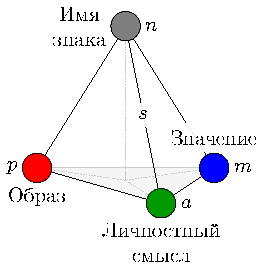
\includegraphics[width=0.25\textwidth]{signs/sign_colored}
		\end{center}
	\end{frame}

	\begin{frame}
		\frametitle{Синтаксический уровень модели}
		
		Пространственные и временные отношения определяются на множестве знаков, а точнее на именах знаков. Отношения на множестве имен транслируются с отношений на множествах компонент знаков. Примеры отношений:
		
		\begin{enumerate}
			\item на образах: отношения эквивалентности, включения, сходства, противопоставления,
			\item на личностных смыслах: поглощения, противопоставления, агглютинации,
			\item на значениях: отношения эквивалентности, сходства, ситуационное и сценарное отношения.
		\end{enumerate}
		
	\end{frame}

	\begin{frame}
		\frametitle{Модель картины мира}
		
		\begin{columns}
			\begin{column}{0.55\textwidth}
				\begin{figure}
					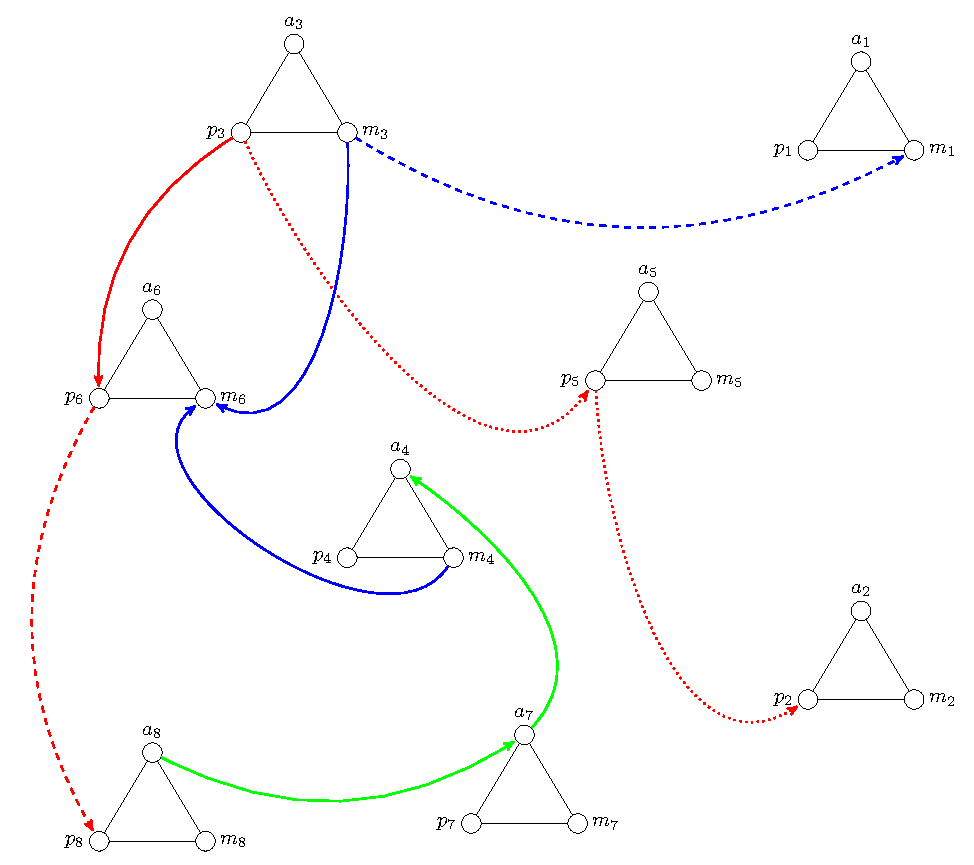
\includegraphics[width=\textwidth]{signs/signs_net}
				\end{figure}
			\end{column}
			\begin{column}{0.45\textwidth}
				\textit{Семиотическая сеть} $H=\langle H_P, H_A, H_M\rangle$, где
				\begin{itemize}
					\item $H_P=\langle2^P,\mathfrak R_P\rangle$ "--- семантическая сеть на множестве образов знаков,
					\item $H_P=\langle2^A,\mathfrak R_A\rangle$ "--- семантическая сеть на множестве значений знаков,
					\item $H_P=\langle2^M,\mathfrak R_M\rangle$ "--- семантическая сеть на множестве личностных смыслов знаков.
				\end{itemize}
			\end{column}
		\end{columns}
	\end{frame}		
	
	\begin{frame}
		\frametitle{Семантический уровень модели}
		
		Для привязки знаков к представляемым объектам  и процессам внешней среды используется иерархия распознающих автоматов. 
		\par\bigskip
		В начальный момент работы автомата поступает управляющий вектор с верхнего уровня иерархии, затем в каждый момент времени $t$ распознающий автомат:
		\begin{enumerate}
			\item векторов действительных чисел от 0 до 1 с нижнего уровня иерархии,
			\item вычисляет текущий весовой вектор выходных признаков и
			\item управляющий вектор на нижний уровень иерархии.
		\end{enumerate}
		
		Состояние автомата $R$ задается множеством битовых матриц предсказания $Z$.
	\end{frame}
	
	\begin{frame}
		\frametitle{Алгоритм $\mathfrak A_{th}$ вычисления автоматной функции}
		
		\begin{tikzpicture}[overlay,remember picture]
		
		\tikzstyle{z_matrix} = [draw, rectangle, minimum width = 60, minimum height = 60,fill=white];
		
		\onslide<1->{
			\node (meas_fun) at (0.7,0.5) {$\hat f_1,\hat f_2\dots,\hat f_k$};	
		}
		\onslide<2->{
			\node (control_vect) at ($(meas_fun)+(-0.5,1.2)$) {$\hat x^{j+1}$};
			\path[->,thick,red] (control_vect.east)  edge[out = -45, in = 45, right] (meas_fun.north); 
		}
		\onslide<3->{
			\node[z_matrix] (z_1) at ($(meas_fun)+(2.6,-0.5)$) {};
			\node[z_matrix] at ($(z_1)+(0.2,-0.1)$) {};
			\node[z_matrix] at ($(z_1)+(0.4,-0.2)$) {};
			
			\node[z_matrix] at ($(z_1)+(0.9,-0.5)$) {};
			\node[z_matrix] at ($(z_1)+(1.1,-0.6)$) {};
			\node[z_matrix] at ($(z_1)+(1.3,-0.7)$) {};
			
			\path[->,thick,blue] ([xshift=20]meas_fun.south)  edge[out = -90, in = -155, right] ($(z_1)+(-1,-1.2)$);
			\path[->,thick,blue] ([xshift=-25]meas_fun.south)  edge[out = -90, in = -155, right] ($(z_1)+(-0.1,-1.7)$);
			
			\node at ($(z_1)+(-1,1.4)$) {$Z^*$};
			
			\node at ($(z_1)+(0.8,1.4)$) {$Z_1$};
			\node at ($(z_1)+(1.4,1.2)$) {$\ddots$};
			\node at ($(z_1)+(2,0.9)$) {$Z_k$};
		}
		
		\onslide<4->{
			\draw[ultra thick, green!60!black] ($(z_1)+(-0.4,-1.1)$) -- ($(z_1)+(-0.4,0.6)$);
			\draw[ultra thick, green!60!black] ($(z_1)+(0.5,-1.6)$) -- node[right,black] {$z_1^r$} ($(z_1)+(0.5,0.1)$);
			
			\draw[->, thick, green!60!black] ($(z_1)+(-0.1,-3)$) -- node[right,black] {$\bar x(0)$} ($(z_1)+(-0.1,-2)$);
		}
		
		\onslide<5->{
			\node[z_matrix] (z_2) at ($(z_1)+(5,0)$) {};
			\node[z_matrix] at ($(z_2)+(0.2,-0.1)$) {};
			
			\node[z_matrix] at ($(z_2)+(0.9,-0.5)$) {};
			\node[z_matrix] at ($(z_2)+(1.3,-0.7)$) {};
			
			\node at ($(z_2)+(-1,1.4)$) {$Z^*$};
			\node at ($(z_2)+(0.8,1.4)$) {$Z_1$};
			\node at ($(z_2)+(1.4,1.2)$) {$\ddots$};
			\node at ($(z_2)+(2,0.9)$) {$Z_k$};
			
			\draw[->, ultra thick] ($(z_1)+(2.6,-0.6)$) -- node [above] {\scriptsize$\frac{\|\bar z_1^r-\bar x(0)\|}{\|\bar z_1^r\|+\|\bar x(0)\|}$} ($(z_1)+(3.7,-0.6)$);
			
			\draw[ultra thick, dotted, green!60!black] ($(z_2)+(-0.6,-1)$) -- ($(z_2)+(-0.6,0.7)$);
			\draw[ultra thick, dotted, green!60!black] ($(z_2)+(0.5,-1.6)$) -- ($(z_2)+(0.5,0.1)$);
		}
		
		
		\onslide<6->{
			\draw[->, thick, red] ($(z_2)+(0.3,1.4)$) -- node[right,black] {$\bar x^*(0)$} ($(z_2)+(0.3,3)$);
		}
		
		\onslide<7>{
			\draw[<-, thick, red] ($(z_2)+(-0.1,-3)$) -- node[right,black] {$\hat x^j(0)$} ($(z_2)+(-0.1,-2)$);
		}
		
		\onslide<7->{				
			\draw[ultra thick, green!60!black] ($(z_2)+(-0.4,-1)$) -- ($(z_2)+(-0.4,0.7)$);
			\draw[ultra thick, green!60!black] ($(z_2)+(0.7,-1.6)$) -- node[right,black] {$z_2^r$} ($(z_2)+(0.7,0.1)$);	
		}
		\onslide<8->{
			\draw[->, thick, green!60!black] ($(z_2)+(-0.1,-3)$) -- node[right,black] {$\bar x(1)$} ($(z_2)+(-0.1,-2)$);
		}
		
		\onslide<9->{
			\draw[->, ultra thick] ($(z_2)+(2.6,-0.6)$) -- node [above] {\scriptsize$\frac{\|\bar z_1^r-\bar x(1)\|}{\|\bar z_1^r\|+\|\bar x(1)\|}$} ($(z_2)+(3.7,-0.6)$);
		}
		\end{tikzpicture}
	\end{frame}

	\begin{frame}
		\frametitle{Компоненты знака}
		
		Если между множеством знаков и множеством признаков, распознаваемых всеми автоматами иерархии, установлено взаимно-однозначное соответствие (именование), то: 
		
		\begin{itemize}
			\item образом знака $s$, соответствующего признаку $f$, является множество всех признаков, участвующих в распознавании признака $f$, 
			\item значением знака $s$, соответствующего признаку $f$, является множество всех процедурных признаков, условия которых распознаются с помощью признака $f$.
		\end{itemize}

	\end{frame}

	\begin{frame}
		\frametitle{Механизм обучения}
		
		К основным принципам работы механизма обучения относятся: 

		\begin{itemize}
			\item использование иерархии вычислительных узлов с восходящими и нисходящими связями, 
			\item использование Хэббовских правил обучения, 
			\item разделение пространственного и временного группировщиков, 
			\item подавление второстепенной активации для формирования разреженного представления.
		\end{itemize}
		
		Формируемые в результате работы механизма обучения связи задают матрицу предсказания для некоторого выходного признака в модели распознающих автоматов.
	\end{frame}

	\begin{frame}
		\frametitle{Модельная задача}
		
		\begin{figure}
			\includegraphics<1>[width=\textwidth]{examples/wall_ex_st0.png}
			\includegraphics<2>[width=\textwidth]{examples/rita_ex_proc.png}
		\end{figure}
	\end{frame}

	\begin{frame}
		\frametitle{Пример представления знаний}
		
		Действия по перемещению "--- знаки $s_t$ (признаки $f_t$, $t$ "--- тип перемещения), которым соответствуют матрицы предсказания типа $Z_t$, состоящие из трёх столбцов 
		\[
			z_1=(l_x, I), z_2=(l_y, d_u, E), z_3=(l_y, I, t_v)
		\]
		,где 
		\begin{itemize}
			\item $l_x$, $l_y$ "--- признаки, соответствующие категории расстояния в пространственной логике  (например, вплотную, близко, далеко и др.), 
			\item $d_u$ "--- признак, соответствующий категории направления в пространственной логике (например, впереди, слева и др.), 
			\item $t_v$ "--- признак, соответствующий категории времени во временной логике (например, скоро, в будущем и др.),
			\item $I$ "--- признак присутствия самого агента, 
			\item $E$ "--- признак отсутствия препятствия.
		\end{itemize}
	\end{frame}	
	
	\begin{frame}
		\frametitle{Обмен сообщениями}
		
		В процессе составления плана решения задачи, агент может обмениваться сообщениям, в состав которых входят компоненты значения, независящие от внутренних характеристик агента и являющихся обобщенными действиями (семантическая сеть со сценарными и ситуационными отношениями).
	\end{frame}

	\begin{frame}
		\frametitle{Планирование совместного перемещения}
		\scalebox{0.7}{
		\begin{tikzpicture}[xshift=90,yshift=90,framed,overlay,remember picture]
			\onslide<1->{
				\blockp{150}{20}{crosshatch} at (0,0) {};
				\blockp{150}{20}{crosshatch} at (10,0) {};
				
				\blockp{20}{40}{crosshatch} at (1.5,-1.5) {};
				\blockp{20}{40}{crosshatch} at (2.5,-3) {};
				
				\blockp{40}{20}{crosshatch} at (4.7,-4.5) {};
				\blockp{20}{15}{north west lines} at (6.5,-2) {};				
				
				\blockp{20}{40}{crosshatch} at (6,-3.1) {};
				\blockp{20}{30}{crosshatch} at (7,-1) {};
				
				\node[draw, circle, dotted, very thick, minimum width = 50, text = black] (goal) at (5, -1) {$G$};
				\node[draw, gray, circle, dotted, very thick, minimum width = 30, text = black] (confl_2) at (6.5, -2) {};				
				\node at (7.5, -2) {$obs_2$};

			}
			\onslide<1-4>{
				\node[draw, gray, fill = gray, circle, very thick, minimum width = 20] (obj_2) at (10, -4) {};
				\node at (10, -3.3) {$A_2$};
			}
			\onslide<1-3>{
				\draw[->, very thick, gray] (obj_2) edge (goal);				
			}
			\onslide<1-5>{
				\blockp{20}{20}{north west lines} at (3.4,-4.5) {};				
				\node[draw, gray, circle, dotted, very thick, minimum width = 40, text = black] (confl_1) at (3.3, -4.3) {};
				\node at (2.2, -4.2) {$obs_1$};								
			}
			\onslide<1>{
				\node[draw, gray, fill = gray, circle, very thick, minimum width = 20] (obj_1) at (4, -7.5) {};
				\node at (4, -6.8) {$A_1$};				
				\draw[->, very thick, dotted, gray] (obj_1) edge [bend left, out = 80, in = 150] (goal);
			}
			\onslide<2-7>{
				\node[draw, gray, fill = gray, circle, very thick, minimum width = 20] (obj_1) at (2.7, -5.3) {};
				\node at (2, -5.3) {$A_1$};				
			}
			\onslide<2>{
				\draw[->, very thick, dotted, gray] (obj_1) edge [bend left, out = 10, in = 160] (goal);				
			}			
			\onslide<3>{
				\draw[->, very thick, dashed, gray] (obj_1) edge [bend left, out = -30, in = -120] node[above,black]{$M_1$} (obj_2);				
			}
			\onslide<4>{
				\draw[->, very thick, gray] (obj_2) edge [out =-120,in=-50] (confl_1);
			}						
			\onslide<5-8>{
				\node[draw, gray, fill = gray, circle, very thick, minimum width = 20] (obj_2) at (3.7, -5.5) {};
				\node at (4.4, -5.5) {$A_2$};	
			}						
			\onslide<7>{
				\draw[->, very thick, dotted, gray] (obj_1) edge [bend left, out = 10, in = 160] (goal);
			}						
			\onslide<7-8>{
				\draw[->, very thick, dotted, gray] (obj_2) edge [bend left, out = 30, in = 170] (goal);
			}
			\onslide<8-9>{
				\node[draw, gray, fill = gray, circle, very thick, minimum width = 20] (obj_1) at (4.5, -0.7) {};
				\node at (3.8, -0.7) {$A_1$};	
			}
			\onslide<9>{
				\node[draw, gray, fill = gray, circle, very thick, minimum width = 20] (obj_2) at (5.5, -1.3) {};
				\node at (6.2, -1.3) {$A_2$};	
			}						
		\end{tikzpicture}
		}
	\end{frame}
		
	\begin{frame}
		\centering
		\Huge
		Спасибо за внимание!
		\normalsize
		\par\bigskip
		\par\bigskip
		ФИЦ ИУ РАН, лаб. <<Динамические интеллектуальные системы>>, pan@isa.ru
	\end{frame}
									
	%	\begin{frame}
	%		\frametitle{Цели курса}
	%		
	%		\begin{itemize}
	%			\item
	%		\end{itemize}
	%	\end{frame}
	
\end{document}
	
	
